\documentclass[12pt]{article}
\usepackage[spanish]{babel}
\usepackage{geometry}
\geometry{a4paper, margin=1in}
\usepackage{graphicx}
\usepackage{xcolor}
\usepackage{titlesec}
\usepackage{parskip}
\usepackage{multicol}
\usepackage{cite}
\usepackage{listings}
\usepackage{color}
\usepackage{amsmath}
\usepackage{enumitem}

\lstset{
  language=Python,
  basicstyle=\ttfamily\small,
  keywordstyle=\color{blue},
  commentstyle=\color{gray},
  stringstyle=\color{red},
  breaklines=true,
  showstringspaces=false
}


\definecolor{highlight}{RGB}{255, 255, 0}

\titleformat{\section}{\normalfont\Large\bfseries}{\thesection}{1em}{}
\titleformat{\subsection}{\normalfont\large\bfseries}{\thesubsection}{1em}{}

\begin{document}

% Logos
\begin{minipage}{0.45\textwidth}
    
\includegraphics[width=0.4\textwidth]{inFiles/Figures/epnLogo.jpg}
\end{minipage}
\hfill
\begin{minipage}{0.45\textwidth}
    \raggedleft
    
\includegraphics[width=0.4\textwidth]{inFiles/Figures/FIS_logo.jpg}
\end{minipage}

\vspace{0.5cm}

% Títulos principales
\begin{center}
    \textbf{ESCUELA POLITÉCNICA NACIONAL}\\[0.2cm]
    \textbf{FACULTAD DE INGENIERÍA DE SISTEMAS}\\[0.2cm]
    \textbf{INGENIERÍA EN CIENCIAS DE LA COMPUTACIÓN}
\end{center}

\vspace{0.5cm}
\hrule
\vspace{0.5cm}

% Datos principales
\noindent\textbf{PERÍODO ACADÉMICO:} 2025-A\\[0.2cm]
\noindent\textbf{ASIGNATURA:} ICCD412 Métodos Numéricos \hfill \textbf{GRUPO:} GR2\\[0.2cm]
\noindent\textbf{TIPO DE INSTRUMENTO:} Tarea7\\[0.2cm]
\noindent\textbf{FECHA DE ENTREGA LÍMITE:} {11/05/2025}\\[0.2cm]
\noindent\textbf{ALUMNO:} {Sebastián Chicaiza}

\vspace{0.5cm}
\hrule
\vspace{1cm}


% Secciones
\section*{TEMA}

\begin{center}
    \Large\textbf{Método de Newton, Secante y Posición Falsa}
\end{center}
\vspace{0.5cm}

\section*{OBJETIVOS}
\begin{itemize}
    \item {Aplicar los métodos de posición falsa, secante y Newton-Rahson para encontrar valores aproximados a la raíz de una función no lineal.}
    \item {Comparar la presición y convergencia de los métodos aplicados.}
\end{itemize}
\vspace{0.5cm}
\section*{MARCO TEÓRICO}
La formula de Newton-Raphson para localizar raíces es la más ampliamente utilizada.
Si el valor inicial para la raíz es \(x_i\), entonces se puede trazar una tangente desde el punto \([x_i, f(x)]\) de la curva.
Por lo común, el punto donde esta tangente cruza el eje \(x\) representa una aproximación mejorada de la raíz \cite{chapra2011metodos}.

\[x_{i+1} = x_i - \frac{f(x_i)}{f'(x_i)} \]



\section*{DESARROLLO}

\subsection*{Conjunto de ejercicios}
\begin{enumerate}
    \item Sea \( f(x) = x^2 - 6 \) y \( p_0 = 1 \). Use el método de Newton para encontrar \( p_2 \).
    \[f(x) = x^{2} - 6 \quad \text(y) \quad f'(x) = 2x\]
    \[
    \begin{aligned}
    p_1 &= p_0 - \frac{f(p_0)}{f'(p_0)} \\
        &= 1 - \frac{1^{2} - 6}{2(1)} \\
        &= \frac{7}{2} = 3.5 \\
    p_2 &= p_1 - \frac{f(p_1)}{f'(p_1)} \\
        &= 3.5 - \frac{3.5^{2} - 6}{2(3.5)} \\
        &\approx 2.607143
    \end{aligned}
    \]
    \item Sea \( f(x) = -x^3 - \cos x \) y \( p_0 = -1 \). Use el método de Newton para encontrar \( p_2 \). ¿Se podría usar \( p_0 = 0 \)?

    \[
    \begin{aligned}
    p_1 &= p_0 - \frac{f(p_0)}{f'(p_0)} \\        
        &= -1 - \frac{-(-1)^{3}- \cos{(-1)}}{-3(-1)^{2} + \sen(-1)} \\
        &\approx -0.88 \\
    p_2 &= p_1 - \frac{f(p_1)}{f'(p_1)} \\
        &= (-0.88) - \frac{-(-0.88)^{3} - \cos{(-0.88)}}{-3(-0.88)^{2} + \sen(-0.88)} \\
        &\approx -0.8657
    \end{aligned}
    \]

    No es posible usar \(p_0 = 0\) porque la función derivada \( f(x) = -3x^{2} + \sen{(x)}\) sería igual a 0 y daría una indeterminación.
    
    
    \item Use el método de Newton para encontrar soluciones precisas dentro de \(10^{-4}\) para los siguientes problemas.
    
    \begin{enumerate}
        \item \( x^3 - 2x^2 - 5 = 0, \quad [1,4] \)
        
        \[f(1) = 1^{3} - 2(1)^{2} - 5 = -6\]
        \[f(4) = 4^{3} - 2(4)^{2} - 5 = 27\]

        Como existe un cambio de signo entre las imágenes del intervalo, sacamos la primera aproximación con el método de la bisección.
        \[p_0 = \frac{1+4}{2} = 2.5\]
        
        \begin{center}
        \begin{tabular}{|c|c|c|c|c|c|}
        \hline
        \(p_0\) & \(p_1\) & \(f(p_0)\) & \(f(p_1)\) & \textbf{TOL} \\
        \hline
        2.5 & 2.714286 & -1.875000 & 8.750000 &  0.214286 \\
        2.714286 & 2.690952 & 0.262394 & 11.244902 &  0.023334 \\
        2.690952 & 2.690648 & 0.003337 & 10.959860 &  0.000304 \\
        2.690648 & 2.690647 & 0.000006 & 10.956168 &  1 \(\cdot 10^{-6}\) \\
        \hline 
        \end{tabular}
        \end{center}

        \item \( x^3 + 3x^2 - 1 = 0, \quad [-3,-2] \)
        \[f(-3) = (-3)^3 + 3(-3)^2 - 1 = -1\]
        \[f(-2) = (-2)^3 + 3(-2)^2 - 1 = 3\]
         Como existe un cambio de signo entre las imágenes del intervalo, sacamos la primera aproximación con el método de la bisección.
         \[p_0 = \frac{-2+(-3)}{2} = -2.5\]

        \begin{center}
        \begin{tabular}{|c|c|c|c|c|c|}
        \hline
        \(p_0\) & \(p_1\) & \(f(p_0)\) & \(f(p_1)\) & \textbf{TOL} \\
        \hline
        -2.5 & -3.066667 & 2.125000 & 3.750000 &  0.566667 \\
        -3.066667 & -2.900876 & -1.626966 & 9.813337 &  0.165791 \\
        -2.900876 & -2.879720 & -0.165863 & 7.839989 &  0.021156 \\
        -2.879720 & -2.879385 & -0.002543 & 7.600042 &  0.000335 \\
        -2.879385 & -2.879385 & 0.000002 & 7.596264 &  0 \\
        \hline 
        \end{tabular}
        \end{center}

        \item \( x - \cos x = 0, \quad [0, \pi/2] \)
        
        \[f(0) = 0 - \cos{(0)} = -1\]
        \[f(\frac{\pi}{2}) = \frac{\pi}{2} - \cos{(\frac{\pi}{2})} \approx 1.57\]
        Como existe un cambio de signo entre las imágenes del intervalo, sacamos la primera aproximación con el método de la bisección.

        \begin{center}
        \begin{tabular}{|c|c|c|c|c|c|}
        \hline
        \(p_0\) & \(p_1\) & \(f(p_0)\) & \(f(p_1)\) & \textbf{TOL} \\
        \hline
        \(\pi / 4\) & 0.739536 & 0.078291 & 1.707107 &  0.045862 \\
        0.739536 & 0.739085 & 0.000755 & 1.673945 &  0.000451 \\
        0.739085 & 0.739085 & 0.0 & 1.673612 &  0 \\
        \hline 
        \end{tabular}
        \end{center}

        \[p_0 = \frac{0 + \frac{\pi}{2}}{2} = \frac{\pi}{4}\]


        \item \( x - 0.8 - 0.2\sin x = 0, \quad [0, \pi/2] \)
        \[f(0) = 0 - 0.8 - 0.2\sin{(0)} = -0.8\] 
        \[f(\frac{\pi}{2}) = \frac{\pi}{2} - 0.8 - 0.2\sin{(\frac{\pi}{2})} = 0.57\]
        
        Como existe un cambio de signo entre las imágenes del intervalo, sacamos la primera aproximación con el método de la bisección.
        \[p_0 = \frac{0 + \frac{\pi}{2}}{2} = \frac{\pi}{4}\]
        
        \begin{center}
        \begin{tabular}{|c|c|c|c|c|c|}
        \hline
        \(p_0\) & \(p_1\) & \(f(p_0)\) & \(f(p_1)\) & \textbf{TOL} \\
        \hline
        \(\pi / 4\) & 0.967120 & -0.156023 & 0.858579 &  0.181722 \\
        0.967120 & 0.964335 & 0.002469 & 0.886465 &  0.002785 \\
        0.964335 & 0.964334 & 0.000001 & 0.886007 &  1\(\cdot 10^{-6}\) \\
        \hline 
        \end{tabular}
        \end{center}



    \end{enumerate}

    \item Use los tres métodos en esta sección para encontrar las soluciones dentro de \(10^{-5}\) para los siguientes problemas.
    \begin{enumerate}
        \item \( 3x - e^x = 0 \) para \( 1 \leq x \leq 2 \)
        \[p_0 = \frac{1+2}{2} = 1.5\]
        Usando el método de Newton-Raphson:
        \begin{center}
        \begin{tabular}{|c|c|c|c|c|c|}
        \hline
        \(p_0\) & \(p_1\) & \(f(p_0)\) & \(f(p_1)\) & \textbf{TOL} \\
        \hline
        1.5 & 1.512358 & 0.018311 & -1.481689 &  0.012358 \\
        1.512358 & 1.512135 & -0.000343 & -1.537417 &  0.000223 \\
        1.512135 & 1.512134 & -0.000000 & -1.536406 &  1\(\cdot 10^{-6}\) \\
        \hline 
        \end{tabular}
        \end{center}

        Usando el método de la secante:
        \[p_0 = 1 \quad \text{y} \quad p_1 = 2\]
        
        
        \begin{center}
        \begin{tabular}{|c|c|c|c|c|c|c|}
        \hline
        \(p_0\) & \(p_1\) & \(p_2\)& \(f(p_0)\) & \(f(p_1)\)&\(f(p_2)\) & \textbf{TOL} \\
        \hline
        1.0 & 2.0 & 1.168615 & 0.281718 & -1.389056 & 0.288312 & 0.831385 \\
        2.0 & 1.168615 & 1.311516 & -1.389056 & 0.288312 & 0.222751 & 0.142901 \\
        1.168615 & 1.311516 & 1.797039 & 0.288312 & 0.222751 & -0.640644 & 0.485523 \\
        1.311516 & 1.797039 & 1.436778 & 0.222751 & -0.640644 & 0.103215 & 0.360261 \\
        1.797039 & 1.436778 & 1.486766 & -0.640644 & 0.103215 & 0.037529 & 0.049988 \\
        1.436778 & 1.486766 & 1.515326 & 0.103215 & 0.037529 & -0.004926 & 0.02856 \\
        1.486766 & 1.515326 & 1.512012 & 0.037529 & -0.004926 & 0.000188 & 0.003314 \\
        1.515326 & 1.512012 & 1.512134 & -0.004926 & 0.000188 & 1\(\cdot 10^{-6}\) & 0.000122 \\
        1.512012 & 1.512134 & 1.512135 & 0.000188 & 1\(\cdot 10^{-6}\) & -1\(\cdot 10^{-6}\) & 1\(\cdot 10^{-6}\) \\ 
        \hline 
        \end{tabular}
        \end{center}

        
        Usando el método de la posición falsa:
        \[p_0 = 1 \quad \text{y} \quad p_1 = 2\]

        \begin{center}
        \begin{tabular}{|c|c|c|c|c|c|}
        \hline
        \(p_0\) & \(p_1\) & \(p_2\)& \(f(p_0)\) & \(f(p_1)\) & \textbf{TOL} \\
        \hline
        1.0 & 2.0 & 1.168615 & 0.281718 & -1.389056 &  0.831385 \\
        2.0 & 1.168615 & 1.311516 & -1.389056 & 0.288312 &  0.142901 \\
        2.0 & 1.311516 & 1.406664 & -1.389056 & 0.222751 &  0.095148 \\
        2.0 & 1.406664 & 1.46017 & -1.389056 & 0.137678 &  0.053506 \\
        2.0 & 1.46017 & 1.48741 & -1.389056 & 0.073818 &  0.02724 \\
        2.0 & 1.48741 & 1.500574 & -1.389056 & 0.036612 &  0.013164 \\
        2.0 & 1.500574 & 1.506774 & -1.389056 & 0.01746 &  0.0062 \\
        2.0 & 1.506774 & 1.509658 & -1.389056 & 0.008171 &  0.002884 \\
        2.0 & 1.509658 & 1.510993 & -1.389056 & 0.003791 &  0.001335 \\
        2.0 & 1.510993 & 1.511609 & -1.389056 & 0.001751 &  0.000616 \\
        2.0 & 1.511609 & 1.511893 & -1.389056 & 0.000807 &  0.000284 \\
        2.0 & 1.511893 & 1.512023 & -1.389056 & 0.000371 &  0.00013 \\
        2.0 & 1.512023 & 1.512083 & -1.389056 & 0.000171 &  6\(\cdot 10^{-5}\) \\
        2.0 & 1.512083 & 1.512111 & -1.389056 & 7.9\(\cdot 10^{-5}\) &  2.8\(\cdot 10^{-5}\) \\
        2.0 & 1.512111 & 1.512124 & -1.389056 & 3.6\(\cdot 10^{-5}\) &  1.3\(\cdot 10^{-5}\) \\
        2.0 & 1.512124 & 1.51213 & -1.389056 & 1.6\(\cdot 10^{-5}\) &  6\(\cdot 10^{-6}\) \\
        \hline 
        \end{tabular}
        \end{center}

        \item \( 2x + 3\cos x - e^x = 0 \) para \( 1 \leq x \leq 2 \)
        
        \[p_0 = \frac{1 + 2}{2} = 1.5\]

        Usando el método de Newton-Raphson:


        \begin{center}
        \begin{tabular}{|c|c|c|c|c|}
        \hline
        \(p_0\) & \(p_1\)& \(f(p_0)\) & \(f(p_1)\) & \textbf{TOL} \\
        \hline
        1.5 & 1.268097 & -1.269477 & -5.474174 &  0.231903 \\
        1.268097 & 1.240120 & -0.123595 & -4.417689 &  0.027977 \\
        1.240120 & 1.239715 & -0.001740 & -4.293497 &  0.000405 \\
        1.239715 & 1.239715 & -0.000001 & -4.291703 &  0 \\
        \hline 
        \end{tabular}
        \end{center}
    \end{enumerate}
    
    Usando el método de la secante:
    \[p_0 = 1 \quad \text{y} \quad p_1 = 2\]
    \begin{center}
        \begin{tabular}{|c|c|c|c|c|c|c|}
        \hline
        \(p_0\) & \(p_1\)& \(p_2\)&\(f(p_0)\) & \(f(p_1)\) & \(f(p_2)\)& \textbf{TOL} \\
        \hline
        1.0 & 2.0 & 1.162925 & 0.902625 & -4.637497 & 0.316541 & 0.837075 \\
        2.0 & 1.162925 & 1.21641 & -4.637497 & 0.316541 & 0.098815 & 0.053485 \\
        1.162925 & 1.21641 & 1.240684 & 0.316541 & 0.098815 & -0.004162 & 0.024274 \\
        1.21641 & 1.240684 & 1.239703 & 0.098815 & -0.004162 & 5\(\cdot 10^{-5}\) & 0.000981 \\
        1.240684 & 1.239703 & 1.239715 & -0.004162 & 5\(\cdot 10^{-5}\) & -1\(\cdot 10^{-6}\) & 1.2\(\cdot 10^{-5}\) \\
        1.239703 & 1.239715 & 1.239715 & 5\(\cdot 10^{-5}\) & -1\(\cdot 10^{-6}\) & -1\(\cdot 10^{-6}\) & 0.0 \\
        \hline 
        \end{tabular}
    \end{center}

    Usando el método de la posición falsa:
    \[p_0 = 1 \quad \text{y} \quad p_1 = 2\]

    \begin{center}
        \begin{tabular}{|c|c|c|c|c|c|}
        \hline
        \(p_0\) & \(p_1\)& \(p_2\)&\(f(p_0)\) & \(f(p_1)\) & \textbf{TOL} \\
        \hline
        1.0 & 2.0 & 1.162925 & 0.902625 & -4.637497 &  0.837075 \\
        2.0 & 1.162925 & 1.21641 & -4.637497 & 0.316541 &  0.053485 \\
        2.0 & 1.21641 & 1.232758 & -4.637497 & 0.098815 &  0.016348 \\
        2.0 & 1.232758 & 1.237648 & -4.637497 & 0.029749 &  0.00489 \\
        2.0 & 1.237648 & 1.239102 & -4.637497 & 0.00886 &  0.001454 \\
        2.0 & 1.239102 & 1.239533 & -4.637497 & 0.002629 &  0.000431 \\
        2.0 & 1.239533 & 1.239661 & -4.637497 & 0.00078 &  0.000128 \\
        2.0 & 1.239661 & 1.239699 & -4.637497 & 0.00023 &  3.8\(\cdot 10^{-5}\) \\
        2.0 & 1.239699 & 1.23971 & -4.637497 & 6.7\(\cdot 10^{-5}\) &  1.1\(\cdot 10^{-5}\) \\
        2.0 & 1.23971 & 1.239713 & -4.637497 & 2\(\cdot 10^{-5}\) &  3\(\cdot 10^{-6}\) \\
        \hline 
        \end{tabular}
    \end{center}
    
    \item El polinomio de cuarto grado
    \[
        f(x) = 230x^4 + 18x^3 + 9x^2 - 221x - 9
    \]
    tiene dos ceros reales, uno en \([-1, 0]\) y el otro en \([0, 1]\). Intente aproximar estos ceros dentro de \(10^{-6}\) con:
    \begin{enumerate}
        \item El método de posición falsa
        \begin{itemize}
            \item \([-1, 0]\)
            \begin{center}
            \begin{tabular}{|c|c|c|c|c|c|}
            \hline
            \(p_0\) & \(p_1\)& \(p_2\)&\(f(p_0)\) & \(f(p_1)\) & \textbf{TOL} \\
            \hline
            -1.0 & 0.0 & -0.020362 & 433.0 & -9.0 &  0.020362 \\
            -1.0 & -0.020362 & -0.03043 & 433.0 & -4.496379 &  0.010068 \\
            -1.0 & -0.03043 & -0.03548 & 433.0 & -2.266946 &  0.00505 \\
            -1.0 & -0.03548 & -0.038031 & 433.0 & -1.14803 &  0.002551 \\
            -1.0 & -0.038031 & -0.039324 & 433.0 & -0.582641 &  0.001293 \\
            -1.0 & -0.039324 & -0.03998 & 433.0 & -0.296023 &  0.000656 \\
            -1.0 & -0.03998 & -0.040314 & 433.0 & -0.150597 &  0.000334 \\
            -1.0 & -0.040314 & -0.040484 & 433.0 & -0.076551 &  0.00017 \\
            -1.0 & -0.040484 & -0.04057 & 433.0 & -0.038862 &  8.6\(\cdot 10^{-5}\) \\
            -1.0 & -0.04057 & -0.040614 & 433.0 & -0.019796 &  4.4\(\cdot 10^{-5}\) \\
            -1.0 & -0.040614 & -0.040636 & 433.0 & -0.010041 &  2.2\(\cdot 10^{-5}\) \\
            -1.0 & -0.040636 & -0.040647 & 433.0 & -0.005163 &  1.1\(\cdot 10^{-5}\) \\
            -1.0 & -0.040647 & -0.040653 & 433.0 & -0.002724 &  6\(\cdot 10^{-6}\) \\
            \hline 
            \end{tabular}
            \end{center}
            
            \item \([0, 1]\)
            
            \begin{center}
            \begin{tabular}{|c|c|c|c|c|c|}
            \hline
            \(p_0\) & \(p_1\)& \(p_2\)&\(f(p_0)\) & \(f(p_1)\) & \textbf{TOL} \\
            \hline
            0.0 & 1.0 & 0.25 & -9.0 & 27.0 &  0.75 \\
            1.0 & 0.25 & 0.773763 & 27.0 & -62.507812 &  0.523763 \\
            1.0 & 0.773763 & 0.944885 & 27.0 & -83.830461 &  0.171122 \\
            1.0 & 0.944885 & 0.961111 & 27.0 & -11.265235 &  0.016226 \\
            1.0 & 0.961111 & 0.962306 & 27.0 & -0.855733 &  0.001195 \\
            1.0 & 0.962306 & 0.962392 & 27.0 & -0.061577 &  8.6e-05 \\
            1.0 & 0.962392 & 0.962398 & 27.0 & -0.004277 &  6e-06 \\
            \hline 
            \end{tabular}
            \end{center}
        \end{itemize}
        \item El método de la secante
        \begin{itemize}
            \item \([-1, 0]\)
            \begin{center}
            \begin{tabular}{|c|c|c|c|c|c|c|}
            \hline
            \(p_0\) & \(p_1\)& \(p_2\)&\(f(p_0)\) & \(f(p_1)\) & \(f(p_2)\)&\textbf{TOL} \\
            \hline
            -1.0 & 0.0 & -0.020362 & 433.0 & -9.0 & -4.496379 & 0.020362 \\
            0.0 & -0.020362 & -0.040691 & -9.0 & -4.496379 & 0.007031 & 0.020329 \\
            -0.020362 & -0.040691 & -0.040659 & -4.496379 & 0.007031 & -6.4\(\cdot 10^{-5}\) & 3.2\(\cdot 10^{-5}\) \\
            -0.040691 & -0.040659 & -0.040659 & 0.007031 & -6.4\(\cdot 10^{-5}\) & -6.4\(\cdot 10^{-5}\) & 0.0 \\
            \hline 
            \end{tabular}
            \end{center}
            \item \([0, 1]\)
            \begin{center}
            \begin{tabular}{|c|c|c|c|c|c|c|}
            \hline
            \(p_0\) & \(p_1\)& \(p_2\)&\(f(p_0)\) & \(f(p_1)\) & \(f(p_2)\)&\textbf{TOL} \\
            \hline
            0.0 & 1.0 & 0.25 & -9.0 & 27.0 & -62.507812 & 0.75 \\
            1.0 & 0.25 & 0.773763 & 27.0 & -62.507812 & -83.830461 & 0.523763 \\
            0.25 & 0.773763 & -1.285423 & -62.507812 & -83.830461 & 879.649987 & 2.059186 \\
            0.773763 & -1.285423 & 0.594597 & -83.830461 & 879.649987 & -104.691386 & 1.88002 \\
            -1.285423 & 0.594597 & 0.394644 & 879.649987 & -104.691386 & -88.129372 & 0.199953 \\
            0.594597 & 0.394644 & -0.669341 & -104.691386 & -88.129372 & 183.724243 & 1.063985 \\
            0.394644 & -0.669341 & 0.049722 & -88.129372 & 183.724243 & -19.962693 & 0.719063 \\
            -0.669341 & 0.049722 & -0.020751 & 183.724243 & -19.962693 & -4.410272 & 0.070473 \\
            0.049722 & -0.020751 & -0.040735 & -19.962693 & -4.410272 & 0.016786 & 0.019984 \\
            -0.020751 & -0.040735 & -0.040659 & -4.410272 & 0.016786 & -6.4e-05 & 7.6e-05 \\
            -0.040735 & -0.040659 & -0.040659 & 0.016786 & -6.4e-05 & -6.4e-05 & 0.0 \\
            \hline 
            \end{tabular}
            \end{center}
            Observación: si es que se utiliza el método de la secante en el intervalo \([0, 1]\) tomando \(p_0 = 0\) y \(p_1 = 1\), convergue hacia una raíz fuera de este intervalo.
            Pero si es que tomamos un \(p_0\) mas cercano a 1 converge hacia una raíz dentro del intervalo.
            
            Tomando \(p_0 = 0.5\): 
            \begin{center}
            \begin{tabular}{|c|c|c|c|c|c|c|}
            \hline
            \(p_0\) & \(p_1\)& \(p_2\)&\(f(p_0)\) & \(f(p_1)\) & \(f(p_2)\)&\textbf{TOL} \\
            \hline
            0.5 & 1.0 & 0.894221 & -100.625 & 27.0 & -39.491002 & 0.105779 \\
            1.0 & 0.894221 & 0.957046 & 27.0 & -39.491002 & -3.528688 & 0.062825 \\
            0.894221 & 0.957046 & 0.963211 & -39.491002 & -3.528688 & 0.542398 & 0.006165 \\
            0.957046 & 0.963211 & 0.96239 & -3.528688 & 0.542398 & -0.00561 & 0.000821 \\
            0.963211 & 0.96239 & 0.962398 & 0.542398 & -0.00561 & -0.000279 & 8e-06 \\
            \hline 
            \end{tabular}
            \end{center}
        \end{itemize}
        \item El método de Newton
        \begin{itemize}
            \item \([-1, 0]\)
            
        \begin{center}
        \begin{tabular}{|c|c|c|c|c|}
        \hline
        \(p_0\) & \(p_1\)& \(f(p_0)\) & \(f(p_1)\) & \textbf{TOL} \\
        \hline
        -0.5 & -0.150452 & 115.875000 & -331.500000 &  0.349548 \\
        -0.150452 & -0.041817 & 24.510155 & -225.618958 &  0.108635 \\
        -0.041817 & -0.040659 & 0.256687 & -221.725586 &  0.001158 \\
        -0.040659 & -0.040659 & -0.000061 & -221.704346 &  0 \\
        \hline 
        \end{tabular}
        \end{center}
            \item \([0, 1]\)
            
        \begin{center}
        \begin{tabular}{|c|c|c|c|c|}
        \hline
        \(p_0\) & \(p_1\)& \(f(p_0)\) & \(f(p_1)\) & \textbf{TOL} \\
        \hline
        0.5 & -0.705090 & -100.625000 & -83.500000 &  1.205090 \\
        -0.705090 & -0.323791 & 201.836426 & -529.339355 &  0.381299 \\
        -0.323791 & -0.064603 & 65.418396 & -252.397583 &  0.259188 \\
        -0.064603 & -0.040686 & 5.313965 & -222.185547 &  0.023917 \\
        -0.040686 & -0.040659 & 0.005924 & -221.705078 &  2.7e-5 \\
        -0.040659 & -0.040659 & -0.000061 & -221.704346 &  0 \\
        \hline 
        \end{tabular}
        \end{center}
        Observación: con el punto medio entre 0 y 1 que es 0.5 converge en una raíz fuera del intervalo, pero si tomamos el punto 1 como raiz inicial converge en una raíz dentro del intervalo.

        Tomando \(p_0 = 1\)

        \begin{center}
        \begin{tabular}{|c|c|c|c|c|}
        \hline
        \(p_0\) & \(p_1\)& \(f(p_0)\) & \(f(p_1)\) & \textbf{TOL} \\
        \hline
        1.0 & 0.964981 & 27 & 771 &  0.035019 \\
        0.964981 & 0.962412 & 1.729980 & 673.346436 &  0.002569 \\
        0.962412 & 0.962398 & 0.009033 & 666.447876 &  1.4\(\cdot 10^{-5}\) \\
        0.962398 & 0.962398 & -0.000275 & 666.410522 &  0 \\
        \hline 
        \end{tabular}
        \end{center}
        \end{itemize}
        
    \end{enumerate}
    Use los extremos de cada intervalo como aproximaciones iniciales en las partes a) y b) y los puntos medios como la aproximación inicial en la parte c).

    \item La función \( f(x) = \tan \pi x - 6 \) tiene cero en \( \left(\frac{1}{\pi}\right) \arctan(6) \approx 0.447431543 \). Sea \( p_0 = 0 \) y \( p_1 = 0.48 \) y use 10 iteraciones en cada uno de los siguientes métodos para aproximar esta raíz. ¿Cuál método es más eficaz y por qué?
    \begin{enumerate}
        \item Método de bisección
        
            \begin{center}
            \begin{tabular}{|c|c|c|c|c|c|c|}
            \hline
            \(a\) & \(b\)& \(p\)&\(f(a)\) & \(f(b)\) & \(f(p)\)&\textbf{TOL} \\
            \hline
            0.0 & 0.48 & 0.24 & -6.0 & 9.894545 & -5.060937 & 0.24 \\
            0.24 & 0.48 & 0.36 & -5.060937 & 9.894545 & -3.874892 & 0.12 \\
            0.36 & 0.48 & 0.42 & -3.874892 & 9.894545 & -2.105257 & 0.06 \\
            0.42 & 0.48 & 0.45 & -2.105257 & 9.894545 & 0.313752 & 0.03 \\
            0.42 & 0.45 & 0.435 & -2.105257 & 0.313752 & -1.171183 & 0.015 \\
            0.435 & 0.45 & 0.4425 & -1.171183 & 0.313752 & -0.524521 & 0.0075 \\
            0.4425 & 0.45 & 0.44625 & -0.524521 & 0.313752 & -0.13435 & 0.00375 \\
            0.44625 & 0.45 & 0.448125 & -0.13435 & 0.313752 & 0.081674 & 0.001875 \\
            0.44625 & 0.448125 & 0.447187 & -0.13435 & 0.081674 & -0.028295 & 0.000938 \\
            0.447187 & 0.448125 & 0.447656 & -0.028295 & 0.081674 & 0.026201 & 0.000469 \\
            \hline 
            \end{tabular}
            \end{center}

        \item Método de posición falsa
        
            \begin{center}
            \begin{tabular}{|c|c|c|c|c|c|}
            \hline
            \(p_0\) & \(p_1\)& \(p_2\)&\(f(p_0)\) & \(f(p_1)\) & \textbf{TOL} \\
            \hline
            0.0 & 0.48 & 0.181194 & -6.0 & 9.894545 &  0.298806 \\
            0.48 & 0.181194 & 0.286187 & 9.894545 & -5.360106 &  0.104993 \\
            0.48 & 0.286187 & 0.348981 & 9.894545 & -4.742212 &  0.062794 \\
            0.48 & 0.348981 & 0.387052 & 9.894545 & -4.052825 &  0.038071 \\
            0.48 & 0.387052 & 0.410304 & 9.894545 & -3.301085 &  0.023252 \\
            0.48 & 0.410304 & 0.424566 & 9.894545 & -2.545667 &  0.014262 \\
            0.48 & 0.424566 & 0.433336 & 9.894545 & -1.859578 &  0.00877 \\
            0.48 & 0.433336 & 0.438737 & 9.894545 & -1.295176 &  0.005401 \\
            0.48 & 0.438737 & 0.442067 & 9.894545 & -0.86852 &  0.00333 \\
            0.48 & 0.442067 & 0.444121 & 9.894545 & -0.566353 &  0.002054 \\
            \hline 
            \end{tabular}
            \end{center}

        \item Método de la secante
            \begin{center}
            \begin{tabular}{|c|c|c|c|c|c|c|}
            \hline
            \(p_0\) & \(p_1\)& \(p_2\)&\(f(p_0)\) & \(f(p_1)\) & \(f(p_2)\)&\textbf{TOL} \\
            \hline
            0.0 & 0.48 & 0.181194 & -6.0 & 9.894545 & -5.360106 & 0.298806 \\
            0.48 & 0.181194 & 0.286187 & 9.894545 & -5.360106 & -4.742212 & 0.104993 \\
            0.181194 & 0.286187 & 1.091987 & -5.360106 & -4.742212 & -5.702692 & 0.8058 \\
            0.286187 & 1.091987 & -3.692318 & -4.742212 & -5.702692 & -4.55135 & 4.784305 \\
            1.091987 & -3.692318 & -22.605071 & -5.702692 & -4.55135 & -3.081364 & 18.912753 \\
            -3.692318 & -22.605071 & -62.249718 & -4.55135 & -3.081364 & -6.99823 & 39.644647 \\
            -22.605071 & -62.249718 & 8.583024 & -3.081364 & -6.99823 & -9.746611 & 70.832742 \\
            -62.249718 & 8.583024 & -242.611837 & -6.99823 & -9.746611 & -3.271896 & 251.194861 \\
            8.583024 & -242.611837 & -369.549233 & -9.746611 & -3.271896 & 0.413738 & 126.937396 \\
            -242.611837 & -369.549233 & -355.299629 & -3.271896 & 0.413738 & -7.373014 & 14.249604 \\
            \hline 
            \end{tabular}
            \end{center}

        El método de la bisección es el mejor en este caso porque tiene garantizada una convergencia a diferencia de los otros dos métodos.
        Además es el método que da la aproximación mas cercana a la raíz.
    \end{enumerate}

    \item La función descrita por \( f(x) = \ln(x^2 + 1) - e^{0.4x} \cos \pi x \) tiene un número infinito de ceros.
    \begin{enumerate}
        \item Determine, dentro de \(10^{-6}\), el único cero negativo.
            \[a = -1 \quad \text{y} \quad b = 0\]
            \begin{center}
            \begin{tabular}{|c|c|c|c|c|c|c|}
            \hline
            \(a\) & \(b\)& \(p\)&\(f(a)\) & \(f(b)\) & \(f(p)\)&\textbf{TOL} \\
            \hline
            -1.0 & 0.0 & -0.5 & 1.3634672 & -1.0 & 0.2231436 & 0.5 \\
            -0.5 & 0.0 & -0.25 & 0.2231436 & -1.0 & -0.5791921 & 0.25 \\
            -0.5 & -0.25 & -0.375 & 0.2231436 & -0.5791921 & -0.1978023 & 0.125 \\
            -0.5 & -0.375 & -0.4375 & 0.2231436 & -0.1978023 & 0.0113644 & 0.0625 \\
            -0.4375 & -0.375 & -0.40625 & 0.0113644 & -0.1978023 & -0.093992 & 0.03125 \\
            -0.4375 & -0.40625 & -0.421875 & 0.0113644 & -0.093992 & -0.0414504 & 0.015625 \\
            -0.4375 & -0.421875 & -0.4296875 & 0.0113644 & -0.0414504 & -0.0150701 & 0.0078125 \\
            -0.4375 & -0.4296875 & -0.4335938 & 0.0113644 & -0.0150701 & -0.0018586 & 0.0039062 \\
            -0.4375 & -0.4335938 & -0.4355469 & 0.0113644 & -0.0018586 & 0.0047515 & 0.0019531 \\
            -0.4355469 & -0.4335938 & -0.4345703 & 0.0047515 & -0.0018586 & 0.0014459 & 0.0009766 \\
            -0.4345703 & -0.4335938 & -0.434082 & 0.0014459 & -0.0018586 & -0.0002066 & 0.0004883 \\
            -0.4345703 & -0.434082 & -0.4343262 & 0.0014459 & -0.0002066 & 0.0006198 & 0.0002441 \\
            -0.4343262 & -0.434082 & -0.4342041 & 0.0006198 & -0.0002066 & 0.0002066 & 0.0001221 \\
            -0.4342041 & -0.434082 & -0.434143 & 0.0002066 & -0.0002066 & -2\(\cdot 10^{-7}\) & 6.1\(\cdot 10^{-5}\) \\
            -0.4342041 & -0.434143 & -0.4341736 & 0.0002066 & -2\(\cdot 10^{-7}\) & 0.0001034 & 3.05\(\cdot 10^{-5}\) \\
            -0.4341736 & -0.434143 & -0.4341583 & 0.0001034 & -2\(\cdot 10^{-7}\) & 5.16\(\cdot 10^{-5}\) & 1.53\(\cdot 10^{-5}\) \\
            -0.4341583 & -0.434143 & -0.4341506 & 5.16\(\cdot 10^{-5}\) & -2\(\cdot 10^{-7}\) & 2.56\(\cdot 10^{-5}\) & 7.6\(\cdot 10^{-6}\) \\
            -0.4341506 & -0.434143 & -0.4341468 & 2.56\(\cdot 10^{-5}\) & -2\(\cdot 10^{-7}\) & 1.27\(\cdot 10^{-5}\) & 3.8\(\cdot 10^{-6}\) \\
            -0.4341468 & -0.434143 & -0.4341449 & 1.27\(\cdot 10^{-5}\) & -2\(\cdot 10^{-7}\) & 6.3\(\cdot 10^{-6}\) & 1.9\(\cdot 10^{-6}\) \\
            -0.4341449 & -0.434143 & -0.434144 & 6.3\(\cdot 10^{-6}\) & -2\(\cdot 10^{-7}\) & 3.2\(\cdot 10^{-6}\) & 9\(\cdot 10^{-7}\) \\
            \hline 
            \end{tabular}
            \end{center}
        \item Determine, dentro de \(10^{-6}\), los cuatro ceros positivos más pequeños.
        
        \begin{itemize}
            \item primer cero positivo \([0; 0.5]\)
            
            \begin{center}
            \begin{tabular}{|c|c|c|c|c|c|c|}
            \hline
            \(a\) & \(b\)& \(p\)&\(f(a)\) & \(f(b)\) & \(f(p)\)&\textbf{TOL} \\
            \hline
            0.0 & 0.5 & 0.25 & -1.0 & 0.2231436 & -0.7208492 & 0.25 \\
            0.25 & 0.5 & 0.375 & -0.7208492 & 0.2231436 & -0.3130384 & 0.125 \\
            0.375 & 0.5 & 0.4375 & -0.3130384 & 0.2231436 & -0.0572663 & 0.0625 \\
            0.4375 & 0.5 & 0.46875 & -0.0572663 & 0.2231436 & 0.0803955 & 0.03125 \\
            0.4375 & 0.46875 & 0.453125 & -0.0572663 & 0.0803955 & 0.010859 & 0.015625 \\
            0.4375 & 0.453125 & 0.4453125 & -0.0572663 & 0.010859 & -0.0233886 & 0.0078125 \\
            0.4453125 & 0.453125 & 0.4492188 & -0.0233886 & 0.010859 & -0.0063097 & 0.0039062 \\
            0.4492188 & 0.453125 & 0.4511719 & -0.0063097 & 0.010859 & 0.0022635 & 0.0019531 \\
            0.4492188 & 0.4511719 & 0.4501953 & -0.0063097 & 0.0022635 & -0.0020262 & 0.0009766 \\
            0.4501953 & 0.4511719 & 0.4506836 & -0.0020262 & 0.0022635 & 0.0001179 & 0.0004883 \\
            0.4501953 & 0.4506836 & 0.4504395 & -0.0020262 & 0.0001179 & -0.0009541 & 0.0002441 \\
            0.4504395 & 0.4506836 & 0.4505615 & -0.0009541 & 0.0001179 & -0.0004183 & 0.0001221 \\
            0.4505615 & 0.4506836 & 0.4506226 & -0.0004183 & 0.0001179 & -0.00015 & 6.11\(\cdot 10^{-5}\) \\
            0.4506226 & 0.4506836 & 0.4506531 & -0.00015 & 0.0001179 & -1.6\(\cdot 10^{-5}\) & 3.05\(\cdot 10^{-5}\) \\
            0.4506531 & 0.4506836 & 0.4506683 & -1.6\(\cdot 10^{-5}\) & 0.0001179 & \(\cdot 10^{-7}\)\(\cdot 10^{-5}\) & 1.53\(\cdot 10^{-5}\) \\
            0.4506531 & 0.4506683 & 0.4506607 & -1.6\(\cdot 10^{-5}\) & \(\cdot 10^{-7}\)\(\cdot 10^{-5}\) & 1.74\(\cdot 10^{-5}\) & 7.6e-06 \\
            0.4506531 & 0.4506607 & 0.4506569 & -1.6\(\cdot 10^{-5}\) & 1.74\(\cdot 10^{-5}\) & 7\(\cdot 10^{-7}\) & 3.8\(\cdot 10^{-6}\) \\
            0.4506531 & 0.4506569 & 0.450655 & -1.6\(\cdot 10^{-5}\) & 7\(\cdot 10^{-7}\) & -7.7\(\cdot 10^{-6}\) & 1.9\(\cdot 10^{-6}\) \\
            0.450655 & 0.4506569 & 0.450656 & -7.7\(\cdot 10^{-6}\) & 7\(\cdot 10^{-7}\) & -3.3\(\cdot 10^{-6}\) & 1\(\cdot 10^{-6}\) \\
            \hline 
            \end{tabular}
            \end{center}

            \item segundo cero positivo \([1.5; 2]\)
            
            \begin{center}
            \begin{tabular}{|c|c|c|c|c|c|c|}
            \hline
            \(a\) & \(b\)& \(p\)&\(f(a)\) & \(f(b)\) & \(f(p)\)&\textbf{TOL} \\
            \hline
            1.5 & 2.0 & 1.75 & 1.178655 & -0.616103 & -0.0221396 & 0.25 \\
            1.5 & 1.75 & 1.625 & 1.178655 & -0.0221396 & 0.5591096 & 0.125 \\
            1.625 & 1.75 & 1.6875 & 0.5591096 & -0.0221396 & 0.2563059 & 0.0625 \\
            1.6875 & 1.75 & 1.71875 & 0.2563059 & -0.0221396 & 0.1131117 & 0.03125 \\
            1.71875 & 1.75 & 1.734375 & 0.1131117 & -0.0221396 & 0.0443787 & 0.015625 \\
            1.734375 & 1.75 & 1.7421875 & 0.0443787 & -0.0221396 & 0.0108285 & 0.0078125 \\
            1.7421875 & 1.75 & 1.7460938 & 0.0108285 & -0.0221396 & -0.0057303 & 0.0039062 \\
            1.7421875 & 1.7460938 & 1.7441406 & 0.0108285 & -0.0057303 & 0.0025309 & 0.0019531 \\
            1.7441406 & 1.7460938 & 1.7451172 & 0.0025309 & -0.0057303 & -0.0016043 & 0.0009766 \\
            1.7441406 & 1.7451172 & 1.7446289 & 0.0025309 & -0.0016043 & 0.0004621 & 0.0004883 \\
            1.7446289 & 1.7451172 & 1.744873 & 0.0004621 & -0.0016043 & -0.0005712 & 0.0002441 \\
            1.7446289 & 1.744873 & 1.7447509 & 0.0004621 & -0.0005712 & -5.44\(\cdot 10^{-5}\) & 0.000122 \\
            1.7446289 & 1.7447509 & 1.7446899 & 0.0004621 & -5.44\(\cdot 10^{-5}\) & 0.0002039 & 6.1\(\cdot 10^{-5}\) \\
            1.7446899 & 1.7447509 & 1.7447204 & 0.0002039 & -5.44\(\cdot 10^{-5}\) & 7.47\(\cdot 10^{-5}\) & 3.05\(\cdot 10^{-5}\) \\
            1.7447204 & 1.7447509 & 1.7447356 & 7.47\(\cdot 10^{-5}\) & -5.44\(\cdot 10^{-5}\) & 1.04\(\cdot 10^{-5}\) & 1.53\(\cdot 10^{-5}\) \\
            1.7447356 & 1.7447509 & 1.7447432 & 1.04\(\cdot 10^{-5}\) & -5.44\(\cdot 10^{-5}\) & -2.18\(\cdot 10^{-5}\) & 7.7\(\cdot 10^{-6}\) \\
            1.7447356 & 1.7447432 & 1.7447394 & 1.04\(\cdot 10^{-5}\) & -2.18\(\cdot 10^{-5}\) & -5.7\(\cdot 10^{-6}\) & 3.8\(\cdot 10^{-6}\) \\
            1.7447356 & 1.7447394 & 1.7447375 & 1.04\(\cdot 10^{-5}\) & -5.7\(\cdot 10^{-6}\) & 2.3\(\cdot 10^{-6}\) & 1.9\(\cdot 10^{-6}\) \\
            1.7447375 & 1.7447394 & 1.7447385 & 2.3\(\cdot 10^{-6}\) & -5.7\(\cdot 10^{-6}\) & -1.9\(\cdot 10^{-6}\) & 9\(\cdot 10^{-7}\) \\
            \hline 
            \end{tabular}
            \end{center}

            \item tercer cero positivo \( [2; 2.5]\)
            

            \begin{center}
            \begin{tabular}{|c|c|c|c|c|c|c|}
            \hline
            \(a\) & \(b\)& \(p\)&\(f(a)\) & \(f(b)\) & \(f(p)\)&\textbf{TOL} \\
            \hline
            2.0 & 2.5 & 2.25 & -0.616103 & 1.9810015 & 0.0629202 & 0.25 \\
            2.0 & 2.25 & 2.125 & -0.616103 & 0.0629202 & -0.4539669 & 0.125 \\
            2.125 & 2.25 & 2.1875 & -0.4539669 & 0.0629202 & -0.2392965 & 0.0625 \\
            2.1875 & 2.25 & 2.21875 & -0.2392965 & 0.0629202 & -0.0988626 & 0.03125 \\
            2.21875 & 2.25 & 2.234375 & -0.0988626 & 0.0629202 & -0.0205936 & 0.015625 \\
            2.234375 & 2.25 & 2.2421875 & -0.0205936 & 0.0629202 & 0.0205142 & 0.0078125 \\
            2.234375 & 2.2421875 & 2.2382812 & -0.0205936 & 0.0205142 & -0.0002031 & 0.0039062 \\
            2.2382812 & 2.2421875 & 2.2402343 & -0.0002031 & 0.0205142 & 0.0101146 & 0.0019532 \\
            2.2382812 & 2.2402343 & 2.2392578 & -0.0002031 & 0.0101146 & 0.0049458 & 0.0009766 \\
            2.2382812 & 2.2392578 & 2.2387695 & -0.0002031 & 0.0049458 & 0.0023688 & 0.0004883 \\
            2.2382812 & 2.2387695 & 2.2385253 & -0.0002031 & 0.0023688 & 0.001082 & 0.0002442 \\
            2.2382812 & 2.2385253 & 2.2384033 & -0.0002031 & 0.001082 & 0.0004395 & 0.0001221 \\
            2.2382812 & 2.2384033 & 2.2383422 & -0.0002031 & 0.0004395 & 0.0001179 & 6.11\(\cdot 10^{-5}\) \\
            2.2382812 & 2.2383422 & 2.2383117 & -0.0002031 & 0.0001179 & -4.26\(\cdot 10^{-5}\) & 3.05\(\cdot 10^{-5}\) \\
            2.2383117 & 2.2383422 & 2.238327 & -4.26\(\cdot 10^{-5}\) & 0.0001179 & 3.79\(\cdot 10^{-5}\) & 1.52\(\cdot 10^{-5}\) \\
            2.2383117 & 2.238327 & 2.2383194 & -4.26\(\cdot 10^{-5}\) & 3.79\(\cdot 10^{-5}\) & -2.1\(\cdot 10^{-6}\) & 7.6\(\cdot 10^{-6}\) \\
            2.2383194 & 2.238327 & 2.2383232 & -2.1\(\cdot 10^{-6}\) & 3.79\(\cdot 10^{-5}\) & 1.79\(\cdot 10^{-5}\) & 3.8\(\cdot 10^{-6}\) \\
            2.2383194 & 2.2383232 & 2.2383213 & -2.1\(\cdot 10^{-6}\) & 1.79\(\cdot 10^{-5}\) & 7.9\(\cdot 10^{-6}\) & 1.9\(\cdot 10^{-6}\) \\
            2.2383194 & 2.2383213 & 2.2383203 & -2.1\(\cdot 10^{-6}\) & 7.9\(\cdot 10^{-6}\) & 2.7\(\cdot 10^{-6}\) & 9\(\cdot 10^{-7}\) \\
            \hline 
            \end{tabular}
            \end{center}



            \item cuarto cero positivo \([3.5; 4]\)

            \begin{center}
            \begin{tabular}{|c|c|c|c|c|c|c|}
            \hline
            \(a\) & \(b\)& \(p\)&\(f(a)\) & \(f(b)\) & \(f(p)\)&\textbf{TOL} \\
            \hline
            3.5 & 4.0 & 3.75 & 2.5839976 & -2.1198191 & -0.4568245 & 0.25 \\
            3.5 & 3.75 & 3.625 & 2.5839976 & -0.4568245 & 1.0176286 & 0.125 \\
            3.625 & 3.75 & 3.6875 & 1.0176286 & -0.4568245 & 0.2524436 & 0.0625 \\
            3.6875 & 3.75 & 3.71875 & 0.2524436 & -0.4568245 & -0.1112437 & 0.03125 \\
            3.6875 & 3.71875 & 3.703125 & 0.2524436 & -0.1112437 & 0.0685928 & 0.015625 \\
            3.703125 & 3.71875 & 3.7109375 & 0.0685928 & -0.1112437 & -0.0218594 & 0.0078125 \\
            3.703125 & 3.7109375 & 3.7070312 & 0.0685928 & -0.0218594 & 0.0232378 & 0.0039062 \\
            3.7070312 & 3.7109375 & 3.7089843 & 0.0232378 & -0.0218594 & 0.0006569 & 0.0019532 \\
            3.7089843 & 3.7109375 & 3.7099609 & 0.0006569 & -0.0218594 & -0.0106095 & 0.0009766 \\
            3.7089843 & 3.7099609 & 3.7094726 & 0.0006569 & -0.0106095 & -0.0049784 & 0.0004883 \\
            3.7089843 & 3.7094726 & 3.7092284 & 0.0006569 & -0.0049784 & -0.0021607 & 0.0002441 \\
            3.7089843 & 3.7092284 & 3.7091063 & 0.0006569 & -0.0021607 & -0.0007515 & 0.0001221 \\
            3.7089843 & 3.7091063 & 3.7090453 & 0.0006569 & -0.0007515 & -4.73\(\cdot 10^{-5}\) & 6.1\(\cdot 10^{-5}\) \\
            3.7089843 & 3.7090453 & 3.7090148 & 0.0006569 & -4.73\(\cdot 10^{-5}\) & 0.0003048 & 3.05\(\cdot 10^{-5}\) \\
            3.7090148 & 3.7090453 & 3.70903 & 0.0003048 & -4.73\(\cdot 10^{-5}\) & 0.0001293 & 1.53\(\cdot 10^{-5}\) \\
            3.70903 & 3.7090453 & 3.7090376 & 0.0001293 & -4.73\(\cdot 10^{-5}\) & 4.16\(\cdot 10^{-5}\) & 7.7\(\cdot 10^{-6}\) \\
            3.7090376 & 3.7090453 & 3.7090414 & 4.16\(\cdot 10^{-5}\) & -4.73\(\cdot 10^{-5}\) & -2.3\(\cdot 10^{-6}\) & 3.9\(\cdot 10^{-6}\) \\
            3.7090376 & 3.7090414 & 3.7090395 & 4.16\(\cdot 10^{-5}\) & -2.3\(\cdot 10^{-6}\) & 1.96\(\cdot 10^{-5}\) & 1.9\(\cdot 10^{-6}\) \\
            3.7090395 & 3.7090414 & 3.7090404 & 1.96\(\cdot 10^{-5}\) & -2.3\(\cdot 10^{-6}\) & 9.3\(\cdot 10^{-6}\) & 9\(\cdot 10^{-7}\) \\
            \hline 
            \end{tabular}
            \end{center}






        \end{itemize}
        \item Determine una aproximación inicial razonable para encontrar el enésimo cero positivo más pequeño de \( f \). \\
        La función es continua para todo x.

        evaluando en 0:
        \[f(0) = \ln(0^2 + 1) - e^{0.4(0)} \cos \pi (0) = -1 \]
        evaluando en 1:
        \[f(1) = \ln(1^2 + 1) - e^{0.4(1)} \cos \pi (1) = 1.7928\]

        Al ser la función contnua para todo x y existiendo un cambio de signo entre \(f(0)\) y \(f(1)\) entonces asumimos que debe haber al menos una raíz en el intervalo \([0;1]\).


        aproximamos una raíz:

        \[p_0 = \frac{0+1}{2} = 0.5\]

        evaluamos \(p_0\):

        \[f(p_0) = f(0.5) = \ln((0.5)^2 + 1) - e^{0.4(0.5)} \cos \pi (0.5) = 0.0969\]
        \textit{[Sugerencia: Dibuje una gráfica aproximada de \( f \).]}
        \item Use la parte c) para determinar, dentro de \(10^{-6}\), el vigesimoquinto cero positivo más pequeño de \( f \).
    
            \[[a,b] = [14, 15]\]
            \begin{center}
            \begin{tabular}{|c|c|c|c|c|c|c|}
            \hline
            \(a\) & \(b\)& \(p\)&\(f(a)\) & \(f(b)\) & \(f(p)\)&\textbf{TOL} \\
            \hline
            14.0 & 15.0 & 14.5 & -265.1432037 & 408.8493285 & 5.3530423 & 0.5 \\
            14.0 & 14.5 & 14.25 & -265.1432037 & 5.3530423 & -206.0127396 & 0.25 \\
            14.25 & 14.5 & 14.375 & -206.0127396 & 5.3530423 & -114.8997515 & 0.125 \\
            14.375 & 14.5 & 14.4375 & -114.8997515 & 5.3530423 & -57.5028175 & 0.0625 \\
            14.4375 & 14.5 & 14.46875 & -57.5028175 & 5.3530423 & -26.6241016 & 0.03125 \\
            14.46875 & 14.5 & 14.484375 & -26.6241016 & 5.3530423 & -10.755157 & 0.015625 \\
            14.484375 & 14.5 & 14.4921875 & -10.755157 & 5.3530423 & -2.7286959 & 0.0078125 \\
            14.4921875 & 14.5 & 14.4960938 & -2.7286959 & 5.3530423 & 1.3056023 & 0.0039062 \\
            14.4921875 & 14.4960938 & 14.4941407 & -2.7286959 & 1.3056023 & -0.7131869 & 0.0019532 \\
            14.4941407 & 14.4960938 & 14.4951172 & -0.7131869 & 1.3056023 & 0.2957376 & 0.0009765 \\
            14.4941407 & 14.4951172 & 14.4946289 & -0.7131869 & 0.2957376 & -0.2088815 & 0.0004882 \\
            14.4946289 & 14.4951172 & 14.494873 & -0.2088815 & 0.2957376 & 0.0433502 & 0.0002441 \\
            14.4946289 & 14.494873 & 14.494751 & -0.2088815 & 0.0433502 & -0.0827205 & 0.000122 \\
            14.494751 & 14.494873 & 14.494812 & -0.0827205 & 0.0433502 & -0.0196868 & 6.1\(\cdot 10^{-5}\) \\
            14.494812 & 14.494873 & 14.4948425 & -0.0196868 & 0.0433502 & 0.0118313 & 3.05\(\cdot 10^{-5}\) \\
            14.494812 & 14.4948425 & 14.4948273 & -0.0196868 & 0.0118313 & -0.0038762 & 1.53\(\cdot 10^{-5}\) \\
            14.4948273 & 14.4948425 & 14.4948349 & -0.0038762 & 0.0118313 & 0.0039775 & 7.6\(\cdot 10^{-6}\) \\
            14.4948273 & 14.4948349 & 14.4948311 & -0.0038762 & 0.0039775 & \(\cdot 10^{-6}\)\(\cdot 10^{-5}\) & 3.8\(\cdot 10^{-6}\) \\
            14.4948273 & 14.4948311 & 14.4948292 & -0.0038762 & \(\cdot 10^{-6}\)\(\cdot 10^{-5}\) & -0.0019128 & 1.9\(\cdot 10^{-6}\) \\
            14.4948292 & 14.4948311 & 14.4948302 & -0.0019128 & \(\cdot 10^{-6}\)\(\cdot 10^{-5}\) & -0.0008794 & 1\(\cdot 10^{-6}\) \\
            \hline 
            \end{tabular}
            \end{center}
    
    \end{enumerate}
\end{enumerate}

\subsection*{Preguntas de análisis}

\begin{enumerate}
\item La función \(f(x) = x^{1/3}\) tiene raíz en \(x = 0\). Usando el punto de inicio de \(x = 1\) y \(p_0 = 5\), \(p_1 = 0.5\) para el método de secante, compare los resultados de los métodos de secante y Newton.

\begin{itemize}
    \item Método de Newton-Raphson \(p_0 = 1\)
    
        \begin{center}
        \begin{tabular}{|c|c|c|c|c|}
        \hline
        \(p_0\) & \(p_1\)& \(f(p_0)\) & \(f(p_1)\) & \textbf{TOL} \\
        \hline
    1.0 & -2.000003 & 1 & 0.333333 &  3.000003 \\
        \hline 
        \end{tabular}
        \end{center}

        Diverge ya que nos dan como dato que tiene su raíz en  \(x = 0\) y las aproximaciones cada vez se alejan más de la raíz.

    \item Método de la secante
    \begin{center}
        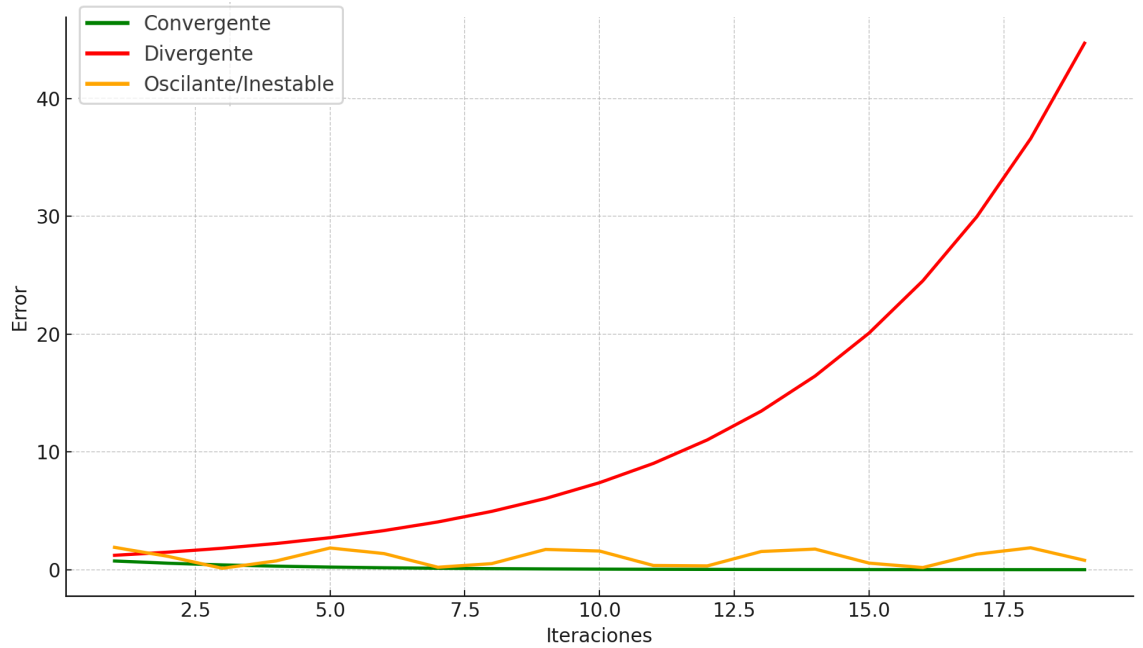
\includegraphics[width=0.9\textwidth]{inFiles/Figures/divergencia.png}
    \end{center}

    La ejecución fracasa ya que diverge y no se cumplirá la condición de parada nunca.
\end{itemize}
\end{enumerate}

\section*{CONCLUSIONES}
\begin{itemize}
    \item {La elección del método a utilizarse depende de la función que deseemos analizar.}
    \item {El método de la secante al no requerir la derivada es una alternativa muy útil aunque no garantiza una converguencia.} 
\end{itemize}

\section*{RECOMENDACIONES}

\begin{itemize}
    \item Usar herramientas de graficación como geogebra.
\end{itemize}

\renewcommand{\refname}{\MakeUppercase{REFERENCIAS}}
\bibliographystyle{IEEEtran}
\bibliography{inFiles/References/references.bib}


\end{document}
